%% FullCourse_10Lecs -- Lecture 10, Topic 10.6b: Case Study 5 --- Inside the Sprint (Execution)
%% Source: ./archive_pre_split/Lec10_Case_Studies_v2.tex (section 6, second half)
%% Pre-emptive sub-split sibling of T6a.
%% Split point: line 2034 of source (sectiondivider for Stages 2, 3, 4 starts T6b).
%% T6b covers: Stage 2 (AI task dispersion), Stage 3 (LLM-built U_o index, 13k tasks),
%%             Stage 4 (exposure refinement, Shapley), and meta-commentary (Agentic AI
%%             under the hood, where skills would tighten the loop, 10 lessons).
%% FullCourse-only content (Case 5 Sprint not in MiniCourse).

%% Shared preamble for the FullCourse_10Lecs topic decks.
%%
%% Each topic .tex \input's this file, then defines its own \title, \date
%% override (if any), \graphicspath, and \begin{document}.
%%
%% Reconstructed verbatim from the inlined copy preserved in
%% Lec10_Case_Studies/Lec10_T8_Case6_DeepRamsey.tex (lines 23-190), which is
%% explicitly annotated there as "from ../shared_preamble.tex, copied verbatim".
%% Base preamble matches MiniCourse_8hr/Slides/shared_preamble.tex; this version
%% additionally provides \sectiondivider, the conceptbox/cautionbox/examplebox/
%% takeawaybox tcolorboxes, and \compacttables used across the split decks.

\documentclass[10pt,english,aspectratio=169]{beamer}

\usepackage{ae,aecompl}
\usepackage[T1]{fontenc}
\usepackage{textcomp}
\usepackage[utf8]{inputenc}
\usepackage{babel}
\usepackage{datetime2}

\setcounter{secnumdepth}{3}
\setcounter{tocdepth}{3}

\usepackage{amsmath, amssymb, amsthm, graphicx}
\usepackage{booktabs, multirow}
\usepackage{tikz}
\usepackage{pgfplots}
\pgfplotsset{compat=1.16}
\usepackage[most]{tcolorbox}
\tcbuselibrary{skins, breakable, theorems}
\usepackage{listings}
\usepackage{xcolor}

\lstset{
  basicstyle=\ttfamily\small,
  keywordstyle=\color{blue!80!black}\bfseries,
  commentstyle=\color{green!50!black}\itshape,
  stringstyle=\color{orange!80!black},
  backgroundcolor=\color{gray!8},
  frame=single,
  rulecolor=\color{gray!40},
  breaklines=true,
  showstringspaces=false,
  numbers=none,
}

\lstdefinestyle{pythonstyle}{
    language=Python,
    basicstyle=\ttfamily\footnotesize,
    keywordstyle=\color{blue!80!black}\bfseries,
    commentstyle=\color{green!50!black}\itshape,
    stringstyle=\color{orange!80!black},
    frame=single,
    breaklines=true,
    showstringspaces=false,
    numbers=left,
    numbersep=5pt,
    numberstyle=\tiny\color{gray},
    backgroundcolor=\color{gray!8},
    rulecolor=\color{gray!40}
}

\ifx\hypersetup\undefined
  \AtBeginDocument{%
    \hypersetup{bookmarks=false,breaklinks=true,pdfborder={0 0 0},colorlinks=true,
      linkcolor=DarkText,urlcolor=RedTitle}%
  }
\else
  \hypersetup{bookmarks=false,breaklinks=true,pdfborder={0 0 0},colorlinks=true,
    linkcolor=DarkText,urlcolor=RedTitle}%
\fi

\makeatletter
\newcommand\makebeamertitle{%
  \begin{frame}[plain]
    \vspace*{1.0cm}
    \centering
    {\usebeamerfont{title}\usebeamercolor[fg]{title}\inserttitle\par}
    \vspace{1.0cm}
    {\usebeamerfont{author}\usebeamercolor[fg]{author}\insertauthor\par}
    \vspace{0.2cm}
    {\usebeamerfont{date}\usebeamercolor[fg]{date}\insertdate\par}
  \end{frame}}%
\AtBeginDocument{%
  \let\origtableofcontents=\tableofcontents
  \def\tableofcontents{\@ifnextchar[{\origtableofcontents}{\gobbletableofcontents}}
  \def\gobbletableofcontents#1{\origtableofcontents}%
}

\usetheme{metropolis}
\usefonttheme{professionalfonts}

\definecolor{LightGray}{RGB}{230,230,230}
\definecolor{RedTitle}{RGB}{0,0,200}
\definecolor{VeryLightGray}{RGB}{245,245,245}
\definecolor{DarkText}{RGB}{0,0,0}

\setbeamercolor{background canvas}{bg=white}
\setbeamercolor{title}{fg=RedTitle}
\setbeamercolor{author}{fg=DarkText}
\setbeamercolor{date}{fg=DarkText}
\setbeamercolor{frametitle}{bg=VeryLightGray,fg=DarkText}
\setbeamercolor{normal text}{fg=DarkText}
\setbeamerfont{title}{size=\large}

\setbeamersize{text margin left=5mm, text margin right=5mm}
\addtobeamertemplate{frametitle}{}{\vspace{-0.5em}}
\newcommand{\reducevspace}{\vspace{-0.5cm}}

% Shared section divider and box styles for split topic decks.
\newcommand{\sectiondivider}[2]{%
\begin{frame}[plain,noframenumbering]
\begin{center}
\vfill
{\Large\textbf{#1}\par}
\vspace{0.35cm}
{\normalsize #2\par}
\vfill
\end{center}
\end{frame}
}

\newtcolorbox{conceptbox}[1][]{
  colback=blue!3,
  colframe=RedTitle!55,
  boxrule=0.35mm,
  arc=1mm,
  left=2mm,
  right=2mm,
  top=1mm,
  bottom=1mm,
  #1
}
\newtcolorbox{cautionbox}[1][]{
  colback=red!3,
  colframe=red!50!black,
  boxrule=0.35mm,
  arc=1mm,
  left=2mm,
  right=2mm,
  top=1mm,
  bottom=1mm,
  #1
}
\newtcolorbox{examplebox}[1][]{
  colback=green!3,
  colframe=green!45!black,
  boxrule=0.35mm,
  arc=1mm,
  left=2mm,
  right=2mm,
  top=1mm,
  bottom=1mm,
  #1
}
\newtcolorbox{takeawaybox}[1][]{
  colback=VeryLightGray,
  colframe=RedTitle!55,
  boxrule=0.35mm,
  arc=1mm,
  left=2mm,
  right=2mm,
  top=1mm,
  bottom=1mm,
  #1
}
\newcommand{\compacttables}{\renewcommand{\arraystretch}{1.15}}

\setbeamertemplate{navigation symbols}{}
\setbeamertemplate{footline}{%
  \hfill%
  \usebeamercolor[fg]{page number in head/foot}%
  \usebeamerfont{page number in head/foot}%
  \insertframenumber\,/\,\inserttotalframenumber\kern1em\vskip2pt%
}

\makeatother

\author{Zhigang Feng}
% "date with time": compile timestamp so each build is identifiable.
\date{\today\ \DTMcurrenttime}


% Suppress redundant auto-generated metropolis section page; \sectiondivider frames are the dividers we keep.
\metroset{sectionpage=none}

\graphicspath{{./pic/}{./figures/}{./Exercise10_ES_Fellows/plots/}{../../MiniCourse_8hr/Slides/Module4_Agentic_AI/pic/}{../}}

\usetikzlibrary{positioning,arrows.meta,shapes,calc,fit,backgrounds}

\lstdefinestyle{markdownstyle}{
    basicstyle=\ttfamily\footnotesize,
    frame=single,
    rulecolor=\color{gray!40},
    backgroundcolor=\color{gray!8},
    breaklines=true,
    showstringspaces=false,
    numbers=none,
}

\title[AI for Econ Research]{AI for Economic Research: Dynamic Models, Language, and Agents\\
Lecture 10.6b: Case Study 5 --- Inside the Sprint (Execution)}

\begin{document}

\makebeamertitle

%=============================================================================
\begin{frame}{Topic 10.6b Agenda}
\begin{enumerate}
  \item \textbf{Inside the Sprint --- Execution} --- Stages 2, 3, 4 and meta-commentary
\end{enumerate}
\end{frame}

%=============================================================================
\section{Case Study 5: Inside the Sprint (Execution)}
%===========================================================

\sectiondivider{Case Study 5 --- Stages 2, 3, 4}{From a single glue index to a distribution --- and an LLM-built index in between}
%===========================================================

% ============================================================
% Frame 5.20 --- Stage 2 opens
% ============================================================
\begin{frame}{Stage 2 --- AI Task Dispersion (opens)}
\begin{columns}[T]
\begin{column}{0.5\textwidth}
\textbf{Question.} Given the mean AI exposure $\bar E_o$, does within-occupation dispersion of exposure predict labor-share movement?

\vspace{0.1cm}
\textbf{Data (new).} Add the \textbf{Eloundou et~al.~(2023)} GPT task-exposure list as a second, independent AI-exposure source parallel to FRS. Tasks, not abilities. 13{,}225 Core tasks across 872 O*NET-SOC codes. We collapse their E0/E1/E2 exposure rubric into \emph{our own} 0--4 $T$-score per task (\emph{our label, not an Eloundou-published variable}).

\vspace{0.1cm}
\textbf{Strategy.} Per-occupation features (\texttt{task\_count}, \texttt{ai\_exposure\_sd}) built at O*NET-SOC, bridged through SOC~2018 $\to$ OCC1950 via CPS-weighted pairs. Outcome: $\Delta$share in an OCC1950 $\times$ (age $\times$ education) cell.
\end{column}
\begin{column}{0.48\textwidth}
\textbf{Report.} Coefficient tables for Experiments A--E across four cells and two sources. Binscatter figures.

\vspace{0.1cm}
\textbf{Analyze.} Nested WLS ladder weighted by pre-period employment share, HC1 SEs:
\begin{itemize}\scriptsize
  \item M0: $\Delta s \sim \bar E$
  \item M1: $\Delta s \sim \bar E + \text{SD}$
  \item M2: $\Delta s \sim \bar E + \text{TC}$
  \item M3: $\Delta s \sim \bar E + \text{SD} + \text{TC}$
\end{itemize}

\vspace{0.1cm}
\textbf{Interpret.} Does $|\hat\beta_{\text{SD}}|$ or $|\hat\beta_{\text{TC}}|$ rival $|\hat\beta_{\bar E}|$ on a 1-SD scale?
\end{column}
\end{columns}

\vspace{0.15cm}
\begin{tcolorbox}[colback=blue!3,colframe=RedTitle!60]\scriptsize
Same six-element template as Stage 1; different question. Pipeline home: \texttt{docs/ai\_task\_dispersion/ai\_task\_dispersion\_memo.tex}, Scripts \texttt{18, 18b, 19, 20, 21}.
\end{tcolorbox}
\end{frame}

% ============================================================
% Frame 5.21 --- Stage 2 Features and Specs
% ============================================================
\begin{frame}{Stage 2 --- Features, Specs, and the Head-to-Head Question}
\begin{columns}[T]
\begin{column}{0.48\textwidth}
\scriptsize
\textbf{Feature pairs per source}
\begin{tabular}{p{2.1cm}p{3.5cm}}
\toprule
\textbf{Source} & \textbf{Features} \\
\midrule
FRS (abilities) & \texttt{task\_count}, \texttt{ai\_exposure\_sd} — 52 abilities screened at IM $\ge 3$ \\
Eloundou (tasks) & \texttt{task\_count\_el}, \texttt{ai\_exposure\_sd\_el} — Core tasks, T-score 0--4 \\
\bottomrule
\end{tabular}

\vspace{0.2cm}
\textbf{The head-to-head.} All features z-scored within cell so the ratio $|\hat\beta_{\text{feat}}/\hat\beta_{\bar E}|$ says ``how many 1-SD of $\bar E$ does a 1-SD of the feature deliver?''
\end{column}
\begin{column}{0.48\textwidth}
\begin{center}
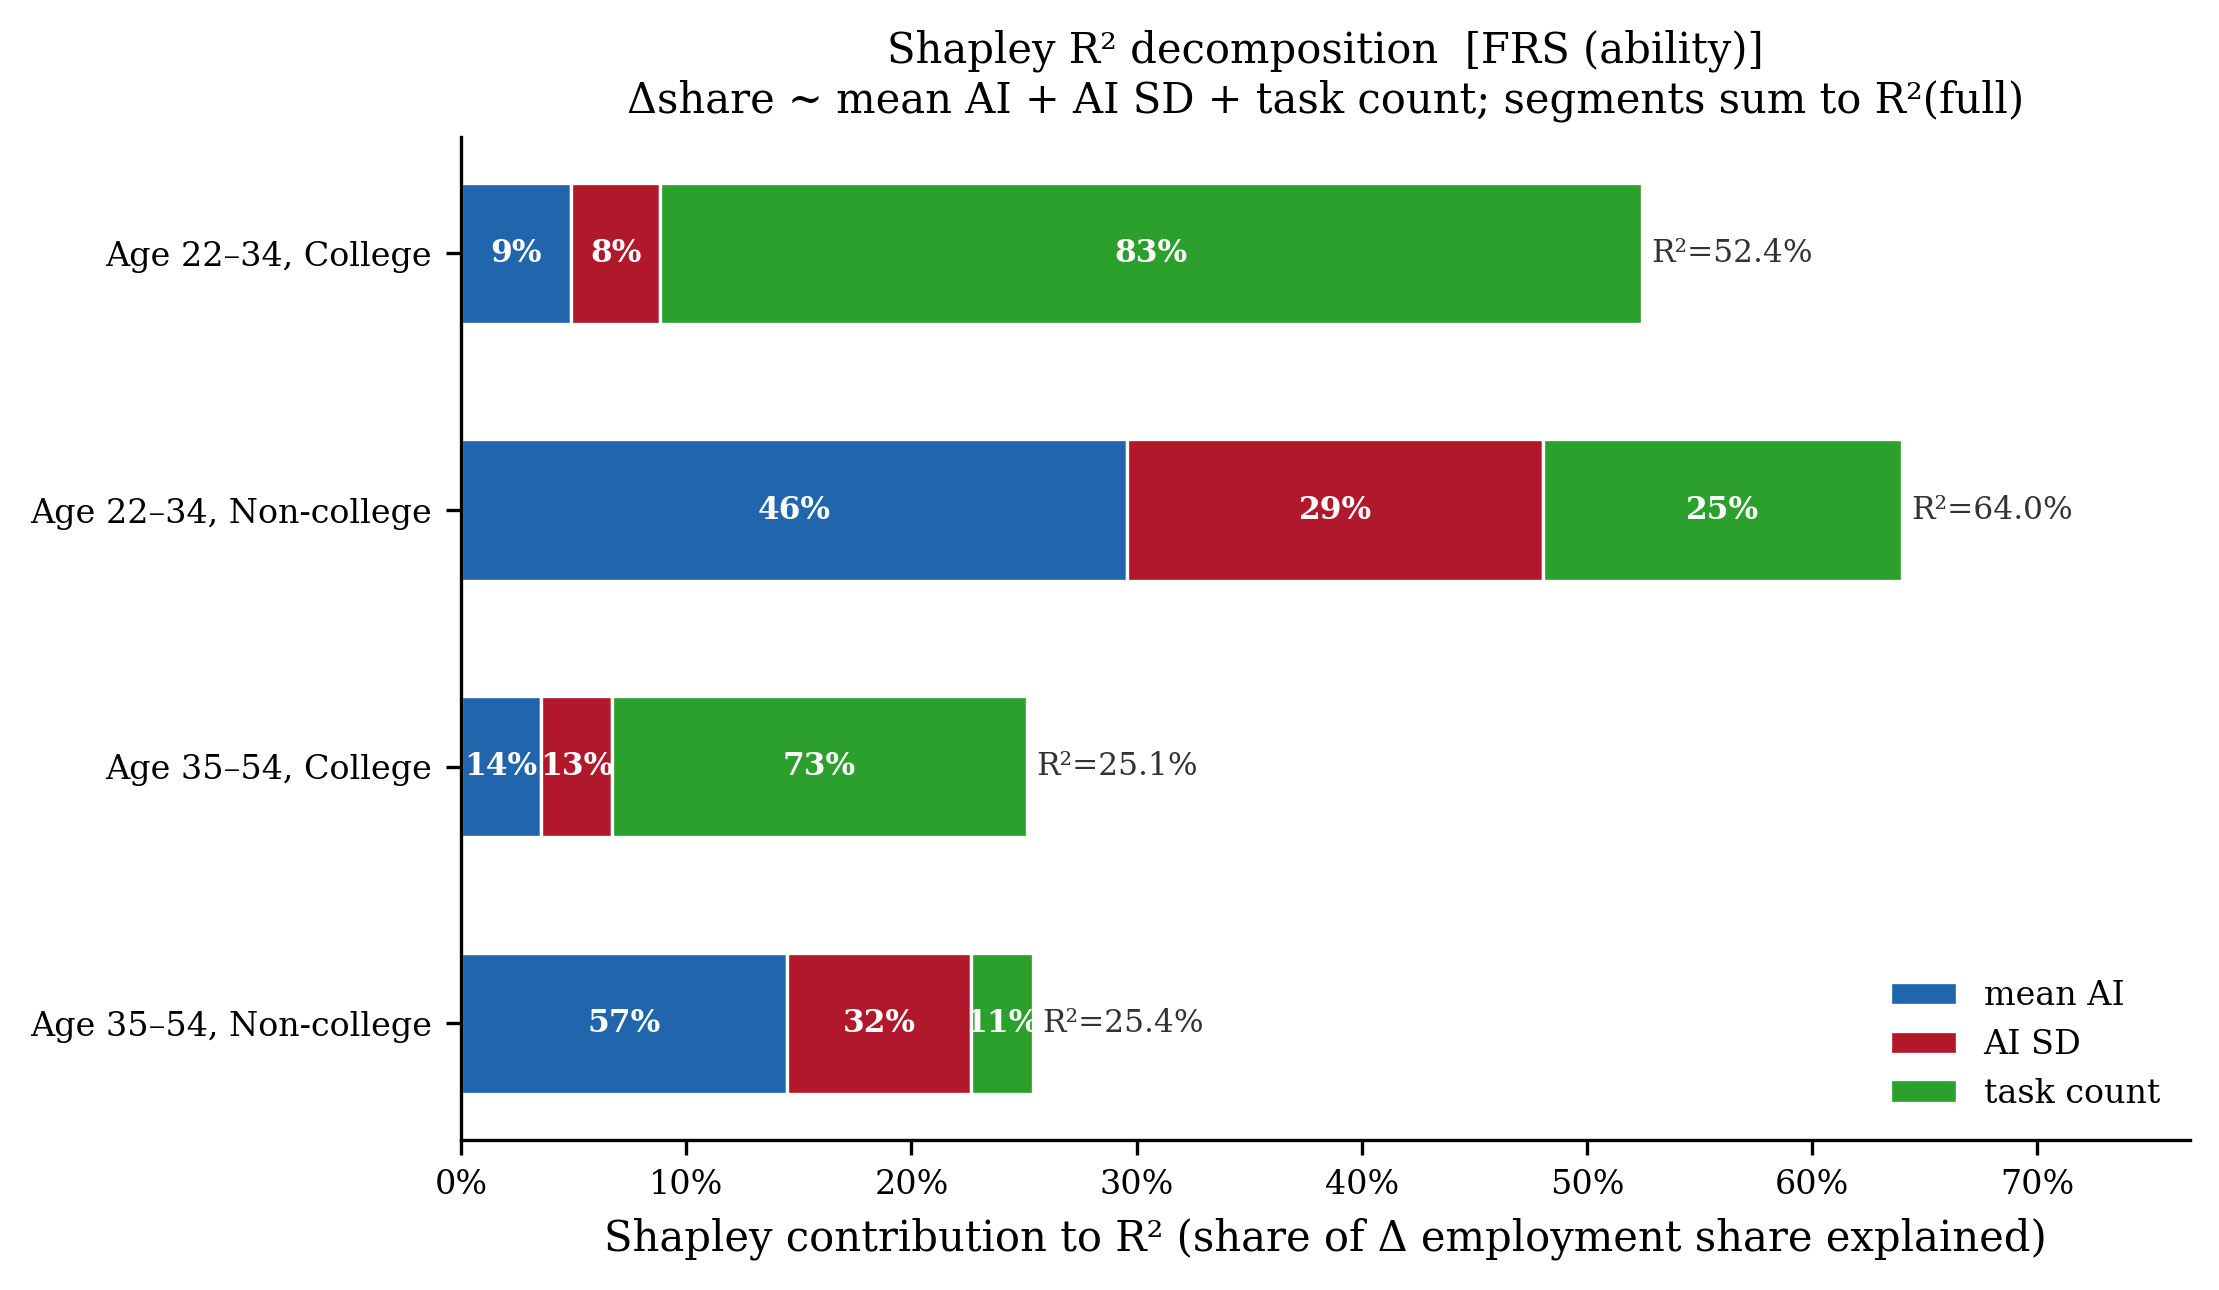
\includegraphics[height=0.58\textheight]{case5/shapley_stacked.png}
\end{center}
\vspace{-0.2cm}
{\scriptsize \textbf{Experiment E Shapley decomposition (FRS side).} Each cell's full-model $R^2$ split across $\{\bar E,\ \text{SD},\ \text{TC}\}$ by average marginal contribution across orderings.}
\end{column}
\end{columns}
\end{frame}

% ============================================================
% Frame 5.22 --- Stage 2 Findings
% ============================================================
\begin{frame}{Stage 2 --- Three Findings}
\begin{enumerate}\small
  \item \textbf{Task count is robust.} Young~$\times$~College: $\hat\beta_{\text{TC}}=+0.0059$ ($p=0.005$) on FRS, $+0.0045$ ($p=0.002$) on Eloundou. Same sign, both sources, same cell. Carries 62--83\% of $R^2$ in the Shapley decomposition for that cell.
  \item \textbf{AI SD is cell-specific.} Significant under Eloundou in Young~$\times$~College ($p=0.018$ in M3) and under FRS in Middle~$\times$~Non-college ($p=0.005$). Elsewhere indistinguishable from zero. Not universal.
  \item \textbf{Mean AI exposure is \emph{not} a sufficient statistic.} In 5 of 8 cells the Shapley share of the mean-AI channel is below half. The residual share is concentrated in TC or SD depending on the cell.
\end{enumerate}

\vspace{0.2cm}
\begin{tcolorbox}[colback=gray!5,colframe=gray!40]\scriptsize
\textbf{Middle $\times$ Non-college (FRS; 36.7\% of prime-age employment).} $\hat\beta_{\bar E} = -0.0040$ (M1), $\hat\beta_{\text{SD}} = -0.0041$ (M1). Ratio $|\hat\beta_{\text{SD}}/\hat\beta_{\bar E}| \approx 1.01$, and SD adds $+15.8$pp to $R^2$ on top of mean AI alone. In this cell, within-job dispersion matches the mean-AI channel dollar-for-dollar.
\end{tcolorbox}
\end{frame}

% ============================================================
% Frame 5.23 --- End of Stage 2
% ============================================================
\begin{frame}{End of Stage 2 --- Memo, Critique, What Launched Stage 3}
\begin{columns}[T]
\begin{column}{0.32\textwidth}
\textbf{The memo}
\begin{tcolorbox}[colback=gray!5,colframe=gray!40]\scriptsize
\texttt{ai\_task\_dispersion\_memo.tex} --- 14 pages, five experiments, descriptive throughout.

\vspace{0.1cm}
Bottom line: the task-count finding survives replication; within-job SD is a second channel with cell-specific bite; mean AI exposure is not a sufficient statistic.
\end{tcolorbox}
\end{column}
\begin{column}{0.32\textwidth}
\textbf{The coauthor critique}
\begin{tcolorbox}[colback=gray!5,colframe=RedTitle!60]\scriptsize
\begin{itemize}\scriptsize
  \item ``Task count tells you the \emph{number} of tasks. But not whether each task is AI-\emph{substitute} or AI-\emph{assist}.''
  \item ``Eloundou gives one $T$-score per task. You need \emph{two}: $e_{\text{sub}}$ and $e_{\text{asst}}$.''
  \item ``Can the LLM itself do this for 13{,}000 tasks?''
\end{itemize}
\end{tcolorbox}
\end{column}
\begin{column}{0.32\textwidth}
\textbf{What launches Stage 3}
\begin{tcolorbox}[colback=blue!3,colframe=RedTitle!60]\small
\emph{Build a task-level LLM-labeled index that decomposes AI exposure into substitution and assistance.}
\end{tcolorbox}
\vspace{0.15cm}\scriptsize
This seeds Scripts 22--29 and the \texttt{unbundling\_vulnerability} track.
\end{column}
\end{columns}
\end{frame}

% ============================================================
% Frame 5.24 --- Stage 3 opens
% ============================================================
\begin{frame}{Stage 3 --- Unbundling Vulnerability (opens)}
\begin{columns}[T]
\begin{column}{0.48\textwidth}
\textbf{The missing decomposition.}

Both FRS AIOE and our Eloundou-based $T$-score deliver \emph{one} number per task or ability. That number bundles two qualitatively different things:
\begin{itemize}\small
  \item $e_{\text{sub}}$ --- AI can \emph{replace} the worker on this task;
  \item $e_{\text{asst}}$ --- AI can \emph{help} the worker do this task faster.
\end{itemize}

\vspace{0.1cm}
A scholar with one task at $e=0.8$ and a call-center agent with one task at $e=0.8$ have the same AIOE score --- and likely very different labor-market trajectories.
\end{column}
\begin{column}{0.48\textwidth}
\textbf{What the LLM can do that the literature can't.}

The O*NET task description plus a rubric is enough for a modern LLM to distinguish the two readings task-by-task. 13{,}225 tasks $\times$ (sub, asst) scores is $\sim$26{,}000 new data points that do not exist in any public release.

\vspace{0.15cm}
\textbf{Deliverables.}
\begin{itemize}\small
  \item $R_o = E_{\text{sub}}/(E_{\text{sub}}+E_{\text{asst}}+\epsilon)$ --- occupation-level substitution share.
  \item $U_o$ --- composite Unbundling Vulnerability Index that uses $R_o$.
\end{itemize}
\end{column}
\end{columns}

\vspace{0.2cm}
\begin{tcolorbox}[colback=blue!3,colframe=RedTitle!60]\scriptsize
\textbf{The LLM can score something the original index was never built to see.} Home: \texttt{docs/unbundling\_vulnerability/}.
\end{tcolorbox}
\end{frame}

% ============================================================
% Frame 5.25 --- The Ambition
% ============================================================
\begin{frame}{Stage 3 --- The Ambition: Scoring 13{,}225 Tasks}
\begin{columns}[T]
\begin{column}{0.5\textwidth}
\scriptsize
\begin{tabular}{lr}
\toprule
Corpus size & \textbf{13{,}225} O*NET Core tasks \\
Per-task output & $(e_{\text{sub}}, e_{\text{asst}}, \text{rationale})$ in $[0,1]$ \\
Calls required (na\"ive) & 13{,}225 LLM calls \\
Budget at Claude Max & one 5-hour window \\
Strategy & \textbf{bulk + adjudicate + cache} \\
\bottomrule
\end{tabular}

\vspace{0.25cm}
\textbf{Three design moves} that turn a 13k-call ambition into a tractable pipeline:
\begin{itemize}\scriptsize
  \item \textbf{Bulk}: 10 tasks per Haiku call --- one JSON array in, one JSON array out. Cuts calls by 10$\times$.
  \item \textbf{Adjudicate}: Sonnet reruns the tasks Haiku flagged as borderline.
  \item \textbf{Cache}: one file per task on disk; re-runs skip already-labeled tasks. Interruption-proof.
\end{itemize}
\end{column}
\begin{column}{0.48\textwidth}
\textbf{Why each move matters}
\begin{tcolorbox}[colback=gray!5,colframe=gray!40]\scriptsize
Without bulking: 13k calls $\times \sim 10$s $= \sim$36~hours --- no single Claude Max window fits.

\vspace{0.1cm}
Without adjudication: Haiku's borderline judgments carry the whole index; no second opinion, no way to flag hard cases.

\vspace{0.1cm}
Without caching: any network blip, quota limit, or power loss destroys hours of work. The 5-hour window \emph{will} expire mid-run --- the cache turns that from a catastrophe into a coffee break.
\end{tcolorbox}
\vspace{0.1cm}
\textbf{Script home.} \texttt{scripts/24\_label\_substitution\_assistance.py}.
\end{column}
\end{columns}
\end{frame}

% ============================================================
% Frame 5.26 --- The Architecture (TikZ flow)
% ============================================================
\begin{frame}{Stage 3 --- The Labeling Architecture}
\begin{center}
\begin{tikzpicture}[
    node distance=0.2cm,
    src/.style={rectangle, rounded corners, draw=gray!60, fill=gray!8,
        minimum width=3.6cm, minimum height=0.5cm, font=\scriptsize, text=DarkText, align=center},
    orch/.style={rectangle, rounded corners, draw=RedTitle, fill=blue!8,
        minimum width=5.2cm, minimum height=0.6cm, font=\scriptsize, text=DarkText, align=center},
    llm/.style={rectangle, rounded corners, draw=orange!80, fill=orange!15,
        minimum width=4.6cm, minimum height=0.55cm, font=\scriptsize, text=DarkText, align=center},
    cache/.style={rectangle, rounded corners, draw=green!60!black, fill=green!10,
        minimum width=4.6cm, minimum height=0.55cm, font=\scriptsize, text=DarkText, align=center},
    agg/.style={rectangle, rounded corners, draw=gray!60, fill=gray!8,
        minimum width=4.6cm, minimum height=0.55cm, font=\scriptsize, text=DarkText, align=center},
    flow/.style={->, gray!70, thick}
]
\node[src] (tasks) {13{,}225 O*NET Core tasks};
\node[orch, below=of tasks] (orch) {Python orchestrator (Script 24)};
\node[llm, below=of orch] (haiku) {Haiku bulk: 10 tasks/call $\to$ JSON array};
\node[cache, below=of haiku] (cache) {Per-task disk cache (resume-safe)};
\node[llm, below=of cache] (sonnet) {Sonnet adjudication on flagged tasks};
\node[agg, below=of sonnet] (agg1) {Script 25: aggregate tasks $\to$ $E_{\text{sub}},\,E_{\text{asst}}$ per occupation};
\node[agg, below=of agg1] (agg2) {Script 26: composite $U_o$};

\draw[flow] (tasks) -- (orch);
\draw[flow] (orch) -- (haiku);
\draw[flow] (haiku) -- (cache);
\draw[flow] (cache) -- (sonnet);
\draw[flow] (sonnet) -- (agg1);
\draw[flow] (agg1) -- (agg2);

\node[right=0.4cm of cache, text=green!60!black, font=\scriptsize\itshape] {resume after 5-h window};
\node[right=0.4cm of haiku, text=orange!80!black, font=\scriptsize\itshape] {``claude --print''};
\end{tikzpicture}
\end{center}

\vspace{-0.05cm}
\begin{tcolorbox}[colback=blue!3,colframe=RedTitle!60]\scriptsize
\textbf{Three layers of LLM.} Claude Code writes Python (layer 1); the Python spawns \texttt{claude --print} Haiku sessions (layer 2); Sonnet adjudicates the borderline cases (layer 3). \textbf{11{,}171 of 13{,}225 tasks labeled (84.5\%)} in one 5-hour window before the quota expired. Resume via cache; no task re-labeled.
\end{tcolorbox}
\end{frame}

% ============================================================
% Frame 5.27 --- The Prompt
% ============================================================
\begin{frame}{Stage 3 --- The Rubric Behind the Labels}
\begin{columns}[T]
\begin{column}{0.48\textwidth}
\textbf{Replacement score $e_{\text{sub}}$}
\begin{itemize}\scriptsize
  \item 0.00: AI cannot replace the task
  \item 0.25: AI handles only narrow pieces
  \item 0.50: human and AI split the task
  \item 0.75: AI does most of the work; human reviews
  \item 1.00: AI replaces the task almost entirely
\end{itemize}
\end{column}
\begin{column}{0.48\textwidth}
\textbf{Assistive score $e_{\text{asst}}$}
\begin{itemize}\scriptsize
  \item 0.00: no productivity gain
  \item 0.25: speeds up a narrow sub-step
  \item 0.50: roughly doubles throughput
  \item 0.75: handles most of the time cost
  \item 1.00: task becomes trivial once AI is used
\end{itemize}
\end{column}
\end{columns}

\vspace{0.12cm}
\begin{tcolorbox}[colback=gray!5,colframe=gray!40]\scriptsize
\textbf{Three anchors.} Clear substitute: \emph{transcribe audio}. Clear assistant: \emph{perform laparoscopic surgery}. Borderline case: \emph{draft a legal contract clause}. Input was a batch of 10 tasks; output was structured JSON with scores, rationale, and an ambiguity flag.
\end{tcolorbox}
\end{frame}

% ============================================================
% Frame 5.28 --- Token engineering detail (tightened)
% ============================================================
\begin{frame}{Stage 3 --- Token Engineering at Scale}
\begin{columns}[T]
\begin{column}{0.48\textwidth}
\scriptsize\textbf{Operational trick}
\begin{tcolorbox}[colback=gray!5,colframe=gray!40]\scriptsize
Run \texttt{claude --print} from a clean temporary directory so the project's 12k-token \texttt{CLAUDE.md} does \emph{not} auto-load into every bulk call.
\end{tcolorbox}

\textbf{Why it matters.} 13k tasks $\Rightarrow$ thousands of repeated calls; small prompt waste becomes massive token waste; cheap calls stay cheap only if context stays minimal.
\end{column}
\begin{column}{0.48\textwidth}
\scriptsize\textbf{Economic interpretation}
\begin{tcolorbox}[colback=blue!3,colframe=RedTitle!60]\scriptsize
\textbf{Saved scale.} About 160M tokens avoided over the full run. At this scale, prompt engineering is not cosmetic; it is cost control and latency control.
\end{tcolorbox}

\textbf{Teaching point.} The rubric stayed constant; the execution environment changed. Agentic AI is strongest when the human specifies the rule once and the system executes it thousands of times.
\end{column}
\end{columns}
\end{frame}

% ============================================================
% Frame 5.29 --- Running Massive Work Unsupervised (tightened)
% ============================================================
\begin{frame}[fragile]{Stage 3 --- Running Massive Work Unsupervised}
\begin{columns}[T]
\begin{column}{0.48\textwidth}
\scriptsize
\textbf{What the economist did.}
\begin{itemize}\scriptsize
  \item Wrote the rubric (\textasciitilde{}30 lines) and three calibration anchors.
  \item Read $\sim$12 LLM-returned labels by eye to sanity-check the scale.
  \item Launched the run and walked away.
\end{itemize}

\textbf{What Claude Code did.}
\begin{itemize}\scriptsize
  \item Wrote the orchestrator (Script 24).
  \item Spawned thousands of \texttt{claude --print} Haiku sessions.
  \item Wrote each task's result to its own cache file.
  \item Detected quota expiration, logged cleanly, exited gracefully.
\end{itemize}

\textbf{What the LLM did.} Returned $(e_{\text{sub}}, e_{\text{asst}})$ for 11{,}171 tasks; flagged 3{,}456 for adjudication.
\end{column}
\begin{column}{0.48\textwidth}
\scriptsize\textbf{Log excerpt} (\texttt{script24\_bulk\_run.log}):
\begin{tcolorbox}[colback=gray!5,colframe=gray!40]
\begin{lstlisting}[style=pythonstyle,numbers=none,basicstyle=\ttfamily\tiny,language={}]
06:41:22 batch 1108 -> 10 cached
...
11:28:03 rate-limit backoff (45s)
11:29:57 ERROR claude-max window expired
11:29:57 cache: 11,171/13,225 tasks
\end{lstlisting}
\end{tcolorbox}
\begin{tcolorbox}[colback=blue!3,colframe=RedTitle!60]\scriptsize
\textbf{Supervision cost.} $\sim 20$ min of economist time to spec the rubric; $\sim 5$ h of unsupervised LLM work; $\sim 12$ labels read by eye out of 11{,}171. This is the ratio that makes LLM labeling a viable empirical tool at corpus scale.
\end{tcolorbox}
\end{column}
\end{columns}
\end{frame}

% ============================================================
% Frame 5.30 --- From Tasks to U_o
% ============================================================
\begin{frame}{Stage 3 --- From per-Task Scores to $U_o$}
\textbf{Task $\to$ occupation aggregation} (Script 25):
\[
E^{\text{sub}}_o = \sum_t w_t \cdot e^{\text{sub}}_t, \quad
E^{\text{asst}}_o = \sum_t w_t \cdot e^{\text{asst}}_t
\]
\[
R_o = \frac{E^{\text{sub}}_o}{E^{\text{sub}}_o + E^{\text{asst}}_o + \epsilon}
\]

\vspace{0.12cm}
\textbf{Composite} (Script 26):
\[
U_o = \alpha\,\bar E_o + \beta\,V_o + \theta\,T_o + \lambda\,(R_o \cdot \bar E_o) - \gamma\,C_o - \mu\,Q_o
\]

\vspace{0.08cm}
\begin{tcolorbox}[colback=gray!5,colframe=gray!40]\scriptsize
\textbf{Interpretation.} $V$ is within-job dispersion, $T$ is top-tail exposure, $C$ is coordination cost, and $Q$ is accountability intensity. The point is not that one scalar is perfect; it is that the index records several reasons a job may be vulnerable or protected.
\end{tcolorbox}
\end{frame}

% ============================================================
% Frame 5.31 --- Weight sensitivity
% ============================================================
\begin{frame}[fragile]{Stage 3 --- Weight Sensitivity of $U_o$}
\begin{columns}[T]
\begin{column}{0.42\textwidth}
\textbf{Declared weights} (\texttt{config.py:AUI\_WEIGHTS}, not data-fit):
\begin{tcolorbox}[colback=gray!5,colframe=gray!40]
\begin{lstlisting}[style=pythonstyle,numbers=none,basicstyle=\ttfamily\tiny,language={}]
AUI_WEIGHTS = {
    "E_bar":     0.30,
    "V":         0.15,
    "T":         0.20,
    "R_times_E": 0.15,
    "C_neg":     0.15,
    "Q_neg":     0.05,
}
\end{lstlisting}
\end{tcolorbox}
\end{column}
\begin{column}{0.54\textwidth}
\begin{center}
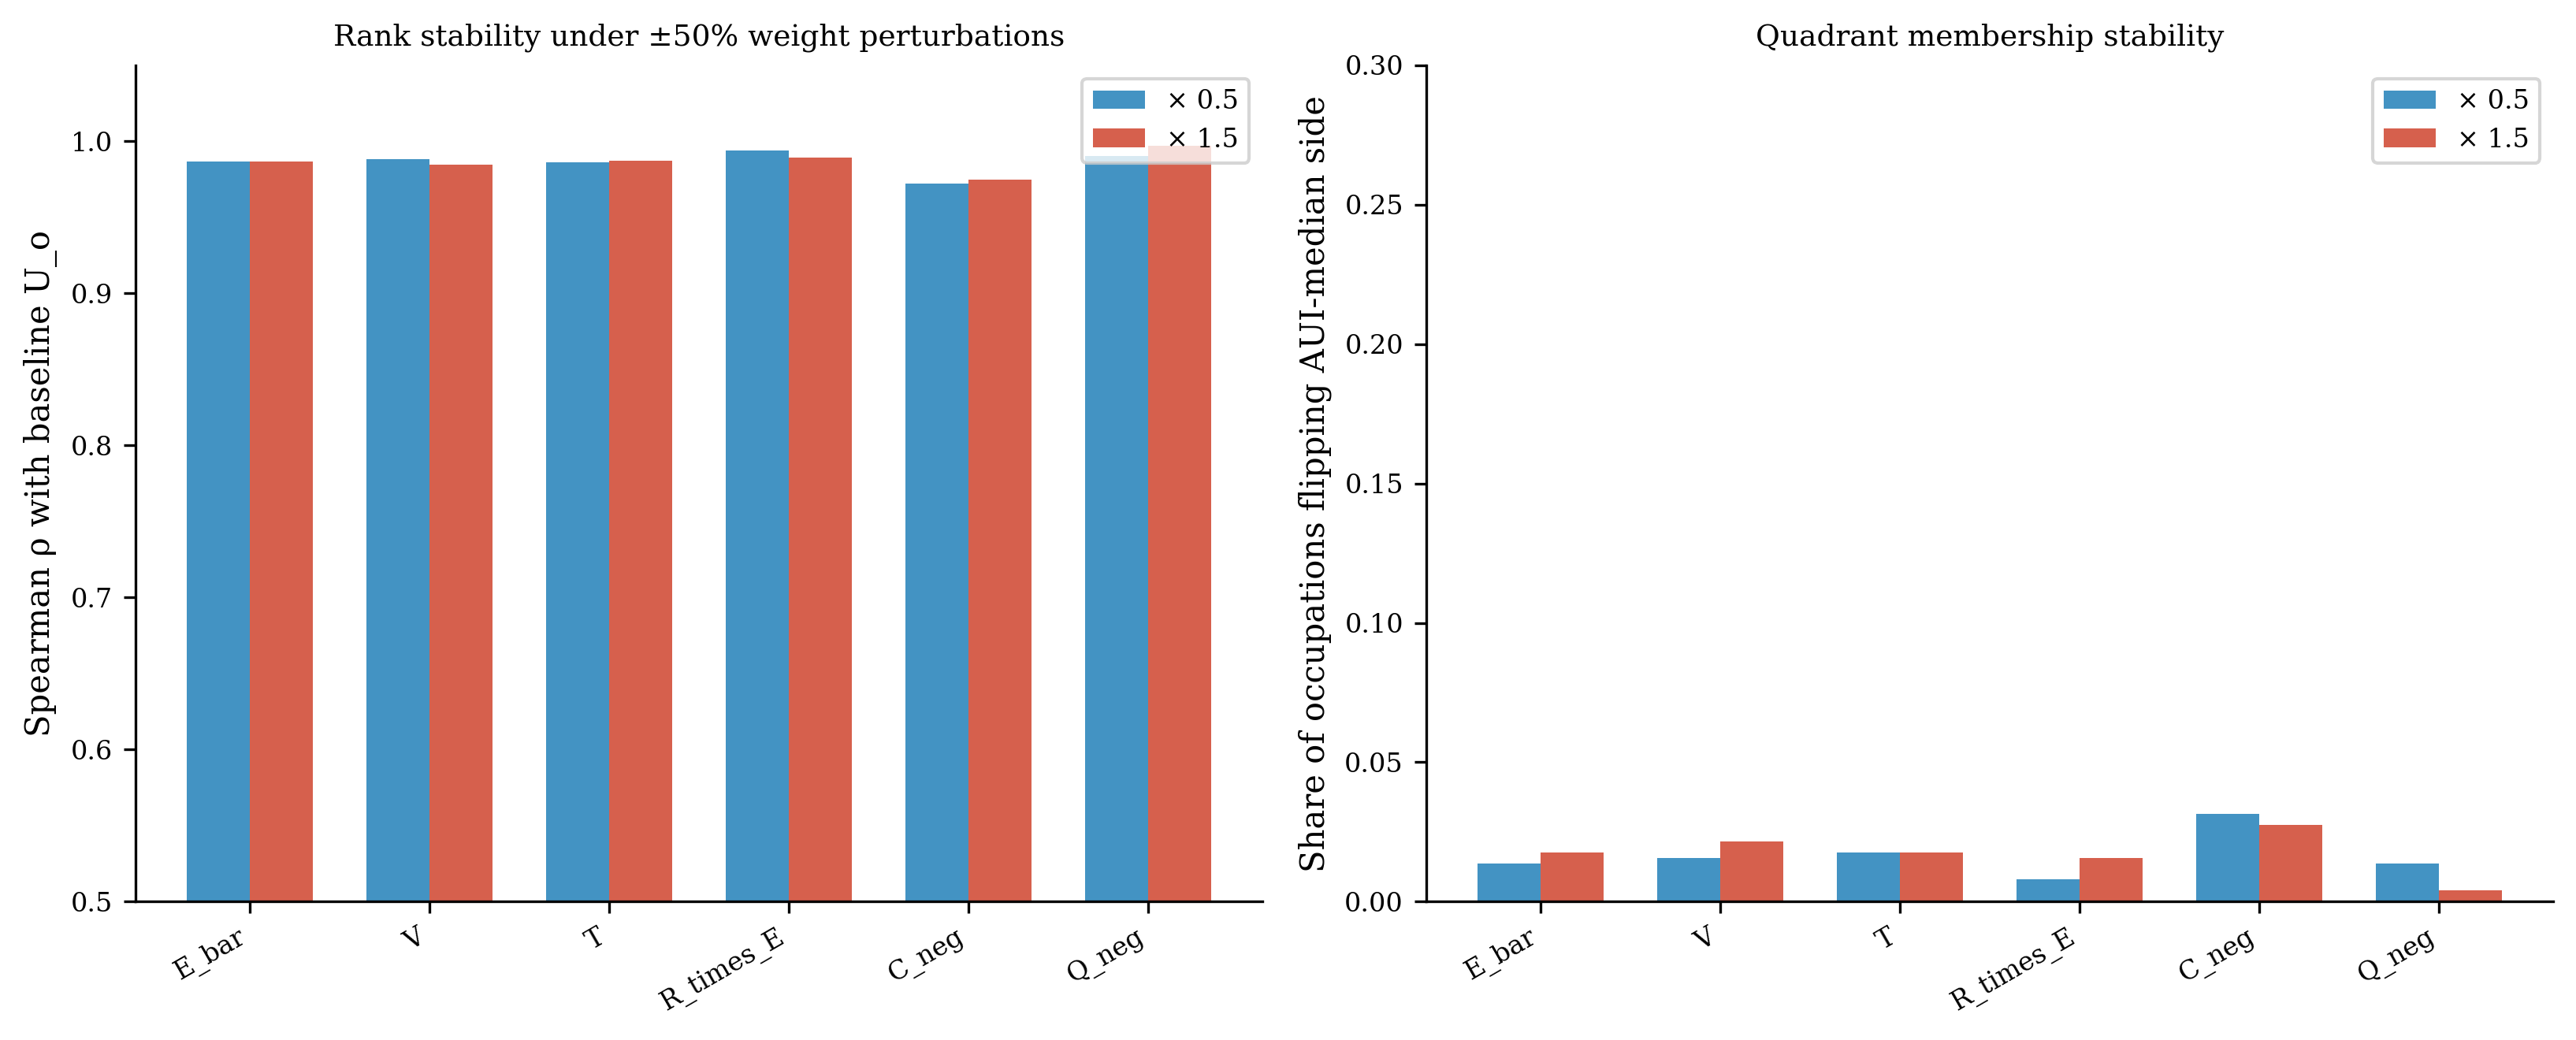
\includegraphics[height=0.52\textheight]{case5/aui_weight_sensitivity.png}
\end{center}
\end{column}
\end{columns}

\vspace{0.08cm}
\begin{tcolorbox}[colback=blue!3,colframe=RedTitle!60]\scriptsize
\textbf{Stability check.} The top and bottom occupations in $U_o$ survive reasonable re-weighting. That does not prove the weights are correct; it shows the ranking is not driven by one arbitrary coefficient choice.
\end{tcolorbox}
\end{frame}

% ============================================================
% Frame 5.32 --- Reading U_o
% ============================================================
\begin{frame}{Stage 3 --- Reading the $U_o$ Index}
\begin{center}
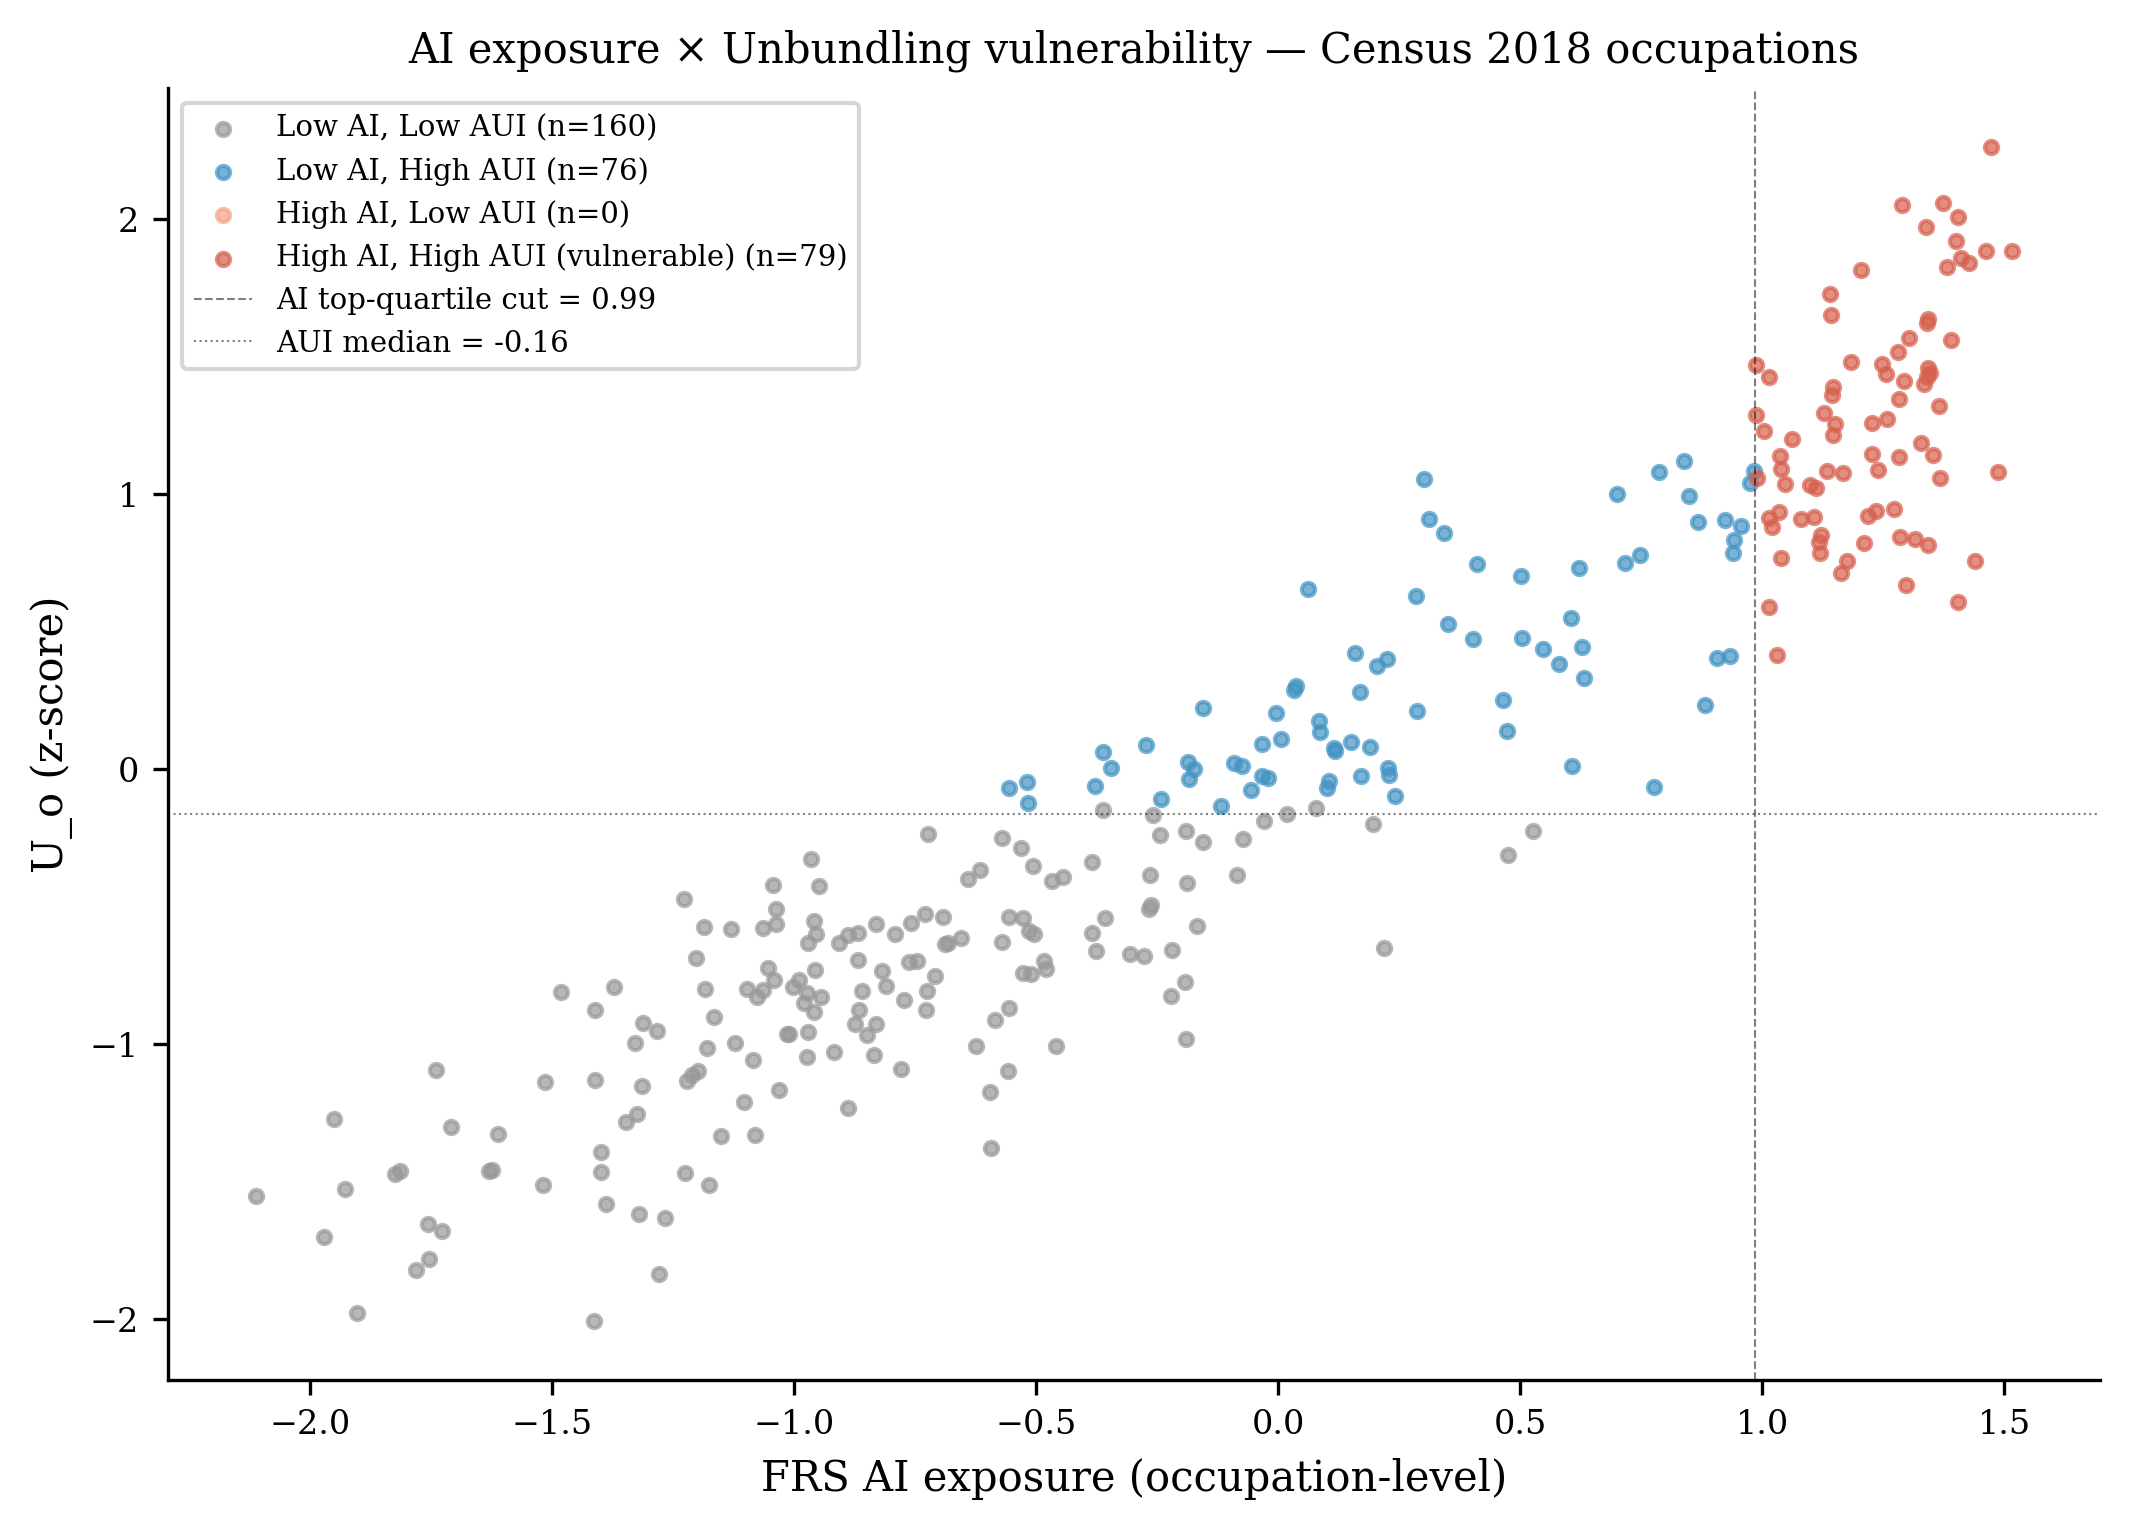
\includegraphics[height=0.60\textheight]{case5/aui_quadrants.png}
\end{center}

\vspace{0.04cm}
\begin{tcolorbox}[colback=blue!3,colframe=RedTitle!60]\scriptsize
\textbf{Quadrants.} Top-right occupations are wholesale-substitution candidates. Top-left occupations face reskilling pressure even when mean exposure is not especially high. The decomposition changes the stories at the margin, not only at the extremes.
\end{tcolorbox}
\end{frame}

% ============================================================
% Frame 5.33 --- Movers under U_o
% ============================================================
\begin{frame}{Stage 3 --- Where $U_o$ Changes the Ranking}
\begin{center}
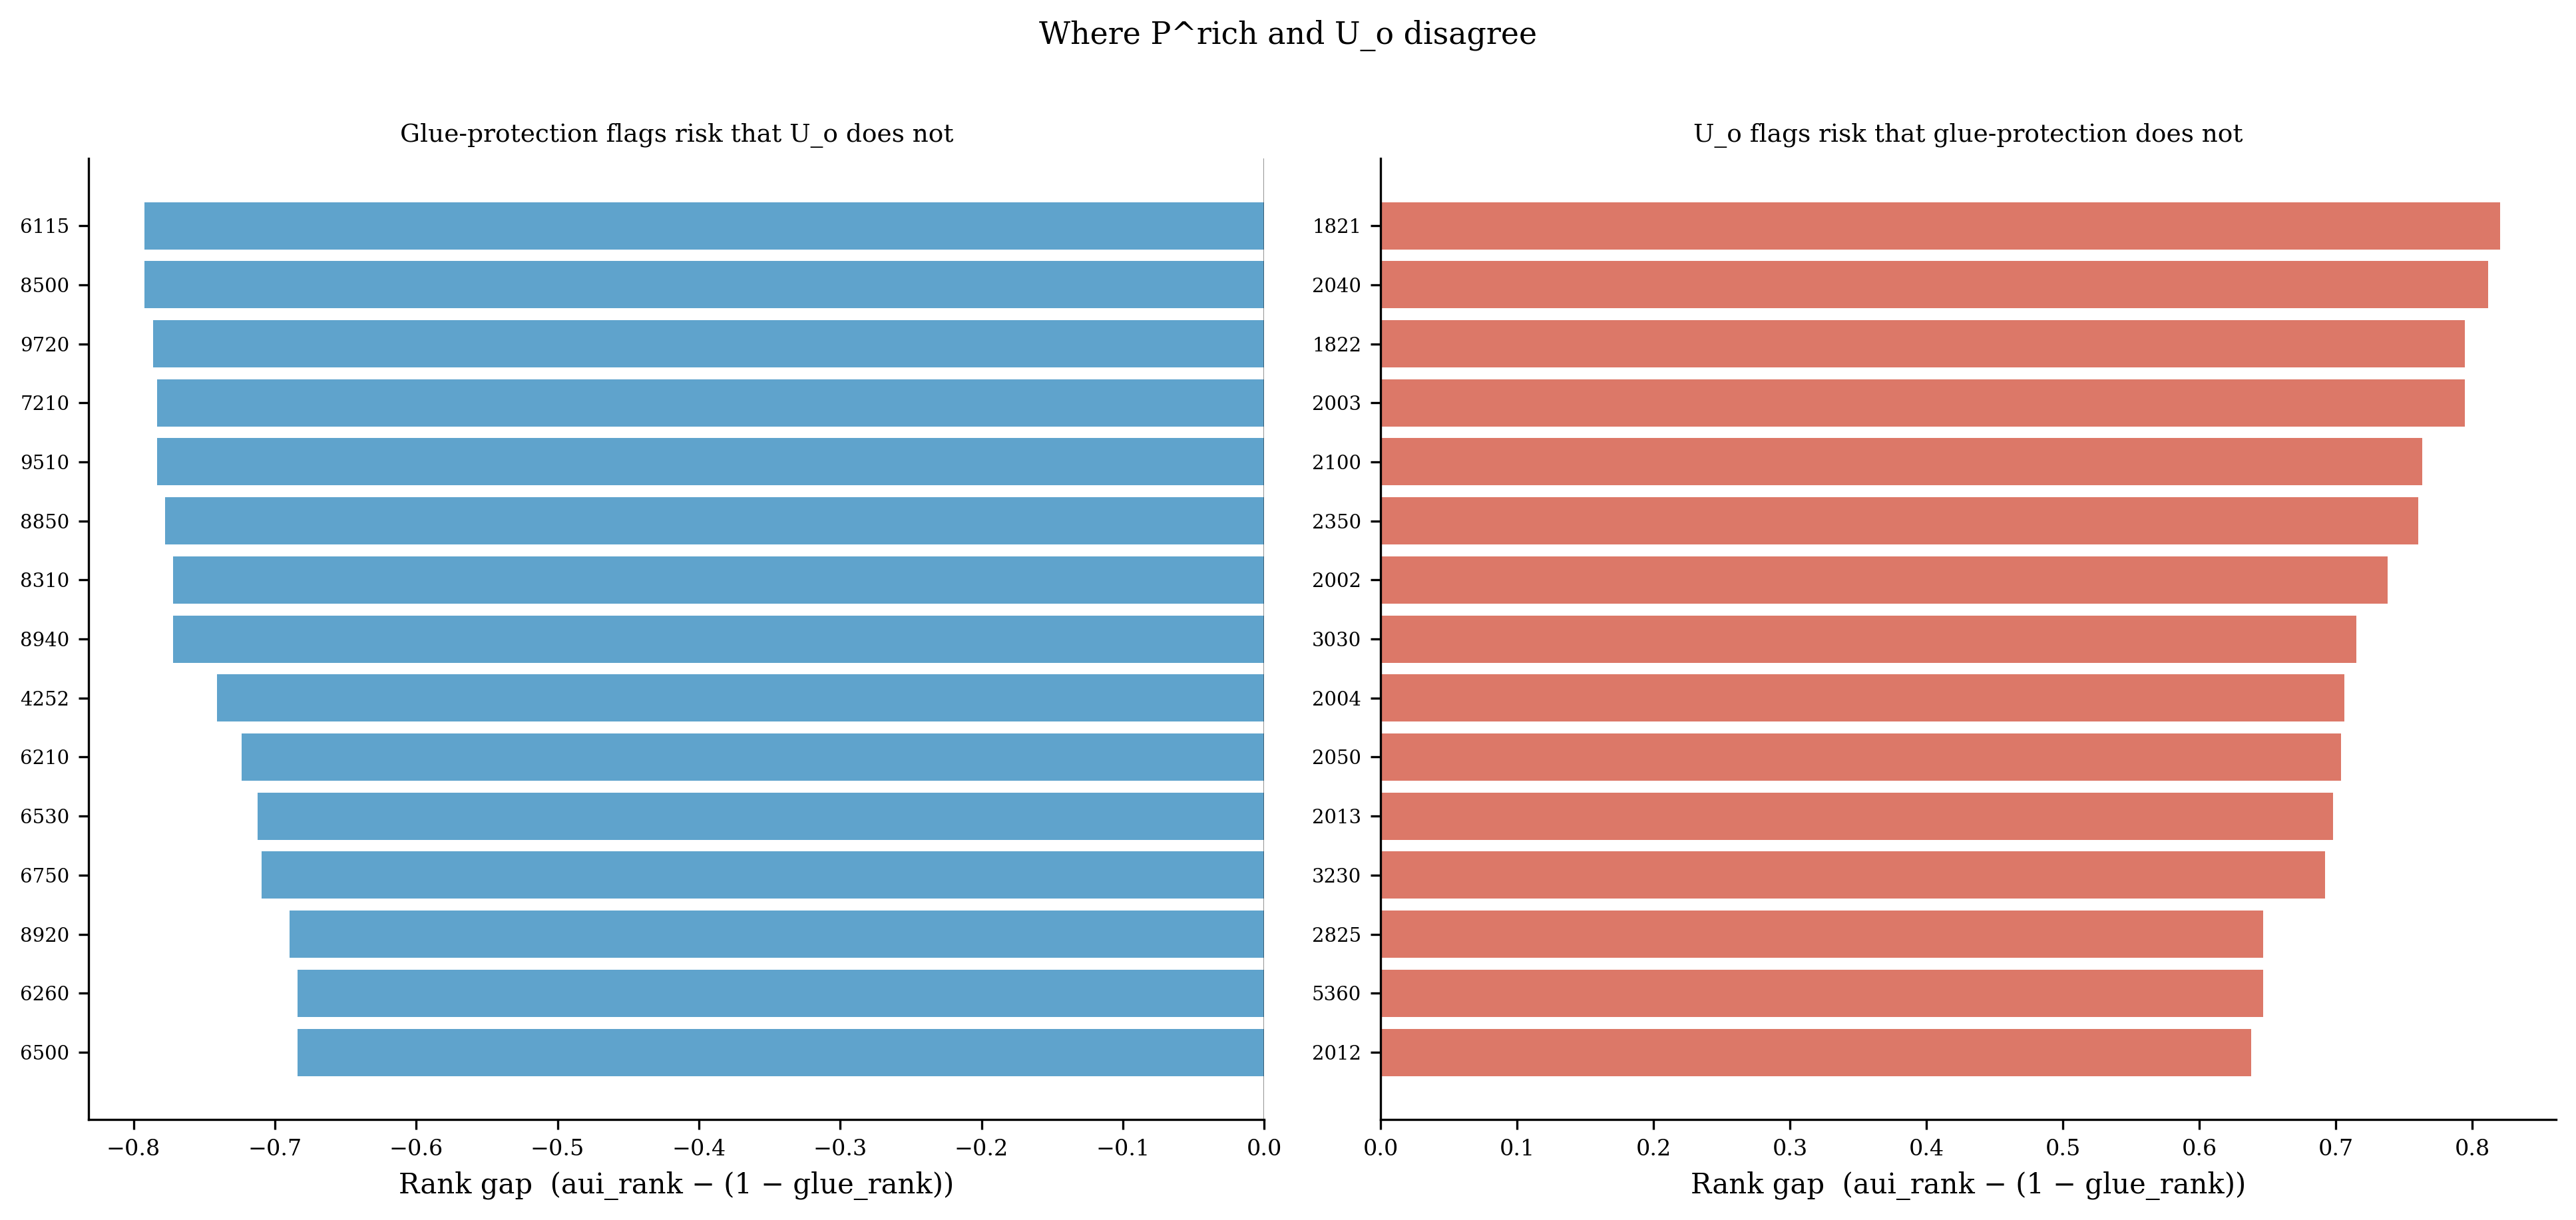
\includegraphics[height=0.68\textheight]{case5/notable_movers.png}
\end{center}

\vspace{0.08cm}
\begin{tcolorbox}[colback=blue!3,colframe=RedTitle!60]\scriptsize
\textbf{Disagreement region.} The interesting cases are where $U_o$ and $P^{\text{rich}}$ disagree. That is exactly where the task-level labeling work pays off: it adds information the Stage 1 protection index could not recover.
\end{tcolorbox}
\end{frame}

% ============================================================
% Frame 5.34 --- End of Stage 3
% ============================================================
\begin{frame}{End of Stage 3 --- Memo, Critique, and Cost}
\begin{columns}[T]
\begin{column}{0.32\textwidth}
\textbf{The memo (partial)}
\begin{tcolorbox}[colback=gray!5,colframe=gray!40]\scriptsize
\texttt{unbundling\_vulnerability\_empirical\_snapshot.md} is populated \emph{partially} because Stage 3 paused with 2{,}054 remainder + 3{,}456 adjudication queued.

\vspace{0.1cm}
The design memo + LLM prompts + quadrant figures are complete; $R_o$ numbers are placeholder pending the remaining labels.
\end{tcolorbox}
\end{column}
\begin{column}{0.32\textwidth}
\textbf{The coauthor critique}
\begin{tcolorbox}[colback=gray!5,colframe=RedTitle!60]\scriptsize
Apr~22 call, Xiaojie Liu:

\vspace{0.1cm}
\emph{``Your top-tail share is 0.97 correlated with mean exposure. You still do not have an independent axis. The within-job \emph{shape of the distribution}, not the upper tail, is where you can learn something $\bar E$ does not carry.''}
\end{tcolorbox}
\end{column}
\begin{column}{0.32\textwidth}
\textbf{What launches Stage 4}
\begin{tcolorbox}[colback=blue!3,colframe=RedTitle!60]\small
\emph{Refine within-job distribution features; test each one against mean AI exposure.}
\end{tcolorbox}

\vspace{0.15cm}
\textbf{Cost accounting.}
\begin{tcolorbox}[colback=gray!5,colframe=gray!40]\scriptsize
$\sim$11k tasks $\times \sim$2 Haiku calls $\times \sim$300 tokens $\approx$ 7M tokens in one 5-h window. Cache guarantees no re-runs.
\end{tcolorbox}
\end{column}
\end{columns}
\end{frame}

% ============================================================
% Frame 5.32 --- Stage 4 opens
% ============================================================
\begin{frame}{Stage 4 --- Exposure Structure Refinement (opens)}
\begin{columns}[T]
\begin{column}{0.48\textwidth}
\textbf{Question.} Holding mean AI exposure $\bar E$ fixed, which \emph{distribution-shape} statistics of within-job exposure add information for labor-share outcomes?

\vspace{0.1cm}
\textbf{Data (no new source).} Same FRS + Eloundou inputs. What changes is the feature set: instead of just mean and SD, compute a family of shape statistics.

\vspace{0.1cm}
\textbf{Strategy.}
\begin{itemize}\scriptsize
  \item Tighten tail thresholds: p33 $\to$ p10 (FRS), $T\ge 3 \to T=4$ (Eloundou).
  \item Add \texttt{top\_bottom\_gap}, \texttt{top\_within\_mean}, \texttt{bottom\_quantile\_mean}, \texttt{importance\_rank\_slope}.
  \item Regress $\Delta$share on each feature (conditioning on $\bar E$), pooled and per-cell.
\end{itemize}
\end{column}
\begin{column}{0.48\textwidth}
\textbf{Report.}
\begin{itemize}\scriptsize
  \item Correlation-with-$\bar E$ table for every feature.
  \item F1 pairwise $\Delta R^2$ rankings.
  \item F5 focused horse race: $\beta(X) / \beta(\bar E)$ ratios.
  \item Shapley-on-4 allocating the increment over the $\bar E$-only baseline.
\end{itemize}

\vspace{0.1cm}
\textbf{Analyze.} Cluster-robust SEs at \texttt{occ1950} for pooled specs (each occupation contributes four cell-rows; HC1 understates). Script \texttt{21b\_run\_exposure\_structure\_regressions.py}.

\vspace{0.1cm}
\textbf{Interpret.} Which refined features beat $\bar E$ in magnitude? Which disappear once $\bar E$ is controlled?
\end{column}
\end{columns}
\end{frame}

% ============================================================
% Frame 5.36 --- Three Archetypes (stylized + real, consolidated)
% ============================================================
\begin{frame}{Stage 4 --- Three Archetypes of Within-Job Exposure}
\begin{columns}[T]
\begin{column}{0.49\textwidth}
\begin{center}
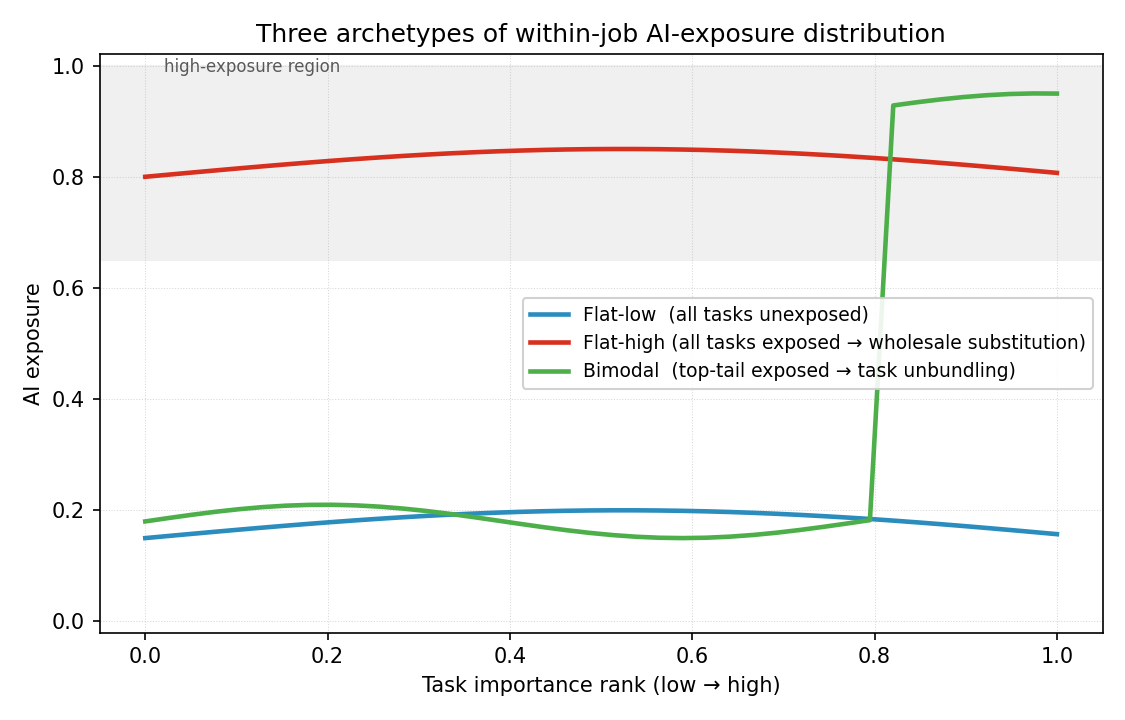
\includegraphics[width=\textwidth]{case5/archetypes_stylized.png}\\
{\scriptsize Stylized}
\end{center}
\end{column}
\begin{column}{0.49\textwidth}
\begin{center}
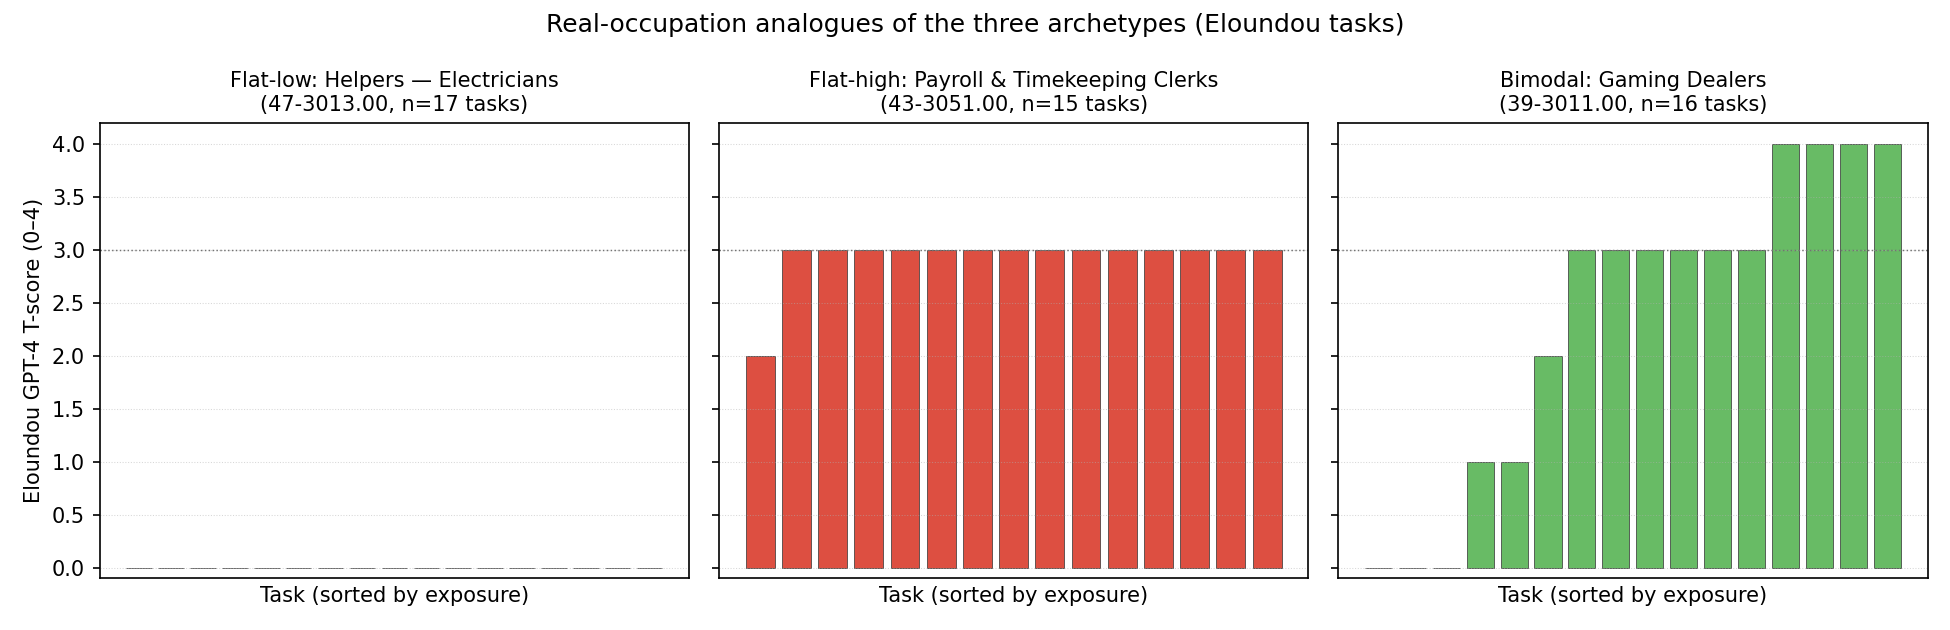
\includegraphics[width=\textwidth]{case5/archetypes_exemplar.png}\\
{\scriptsize Real analogues}
\end{center}
\end{column}
\end{columns}

\vspace{0.08cm}
\begin{tcolorbox}[colback=blue!3,colframe=RedTitle!60]\scriptsize
\textbf{Conceptual point.} Flat-low, flat-high, and bimodal jobs can share the same mean exposure while implying three different labor-market predictions: untouched, wholesale substitution, and unbundling. \textbf{Examples:} Helpers--Electricians look flat-low; Payroll and Timekeeping Clerks look flat-high; Gaming Dealers look bimodal.
\end{tcolorbox}
\end{frame}

% ============================================================
% Frame 5.34 --- Refined feature set
% ============================================================
\begin{frame}[fragile]{Stage 4 --- The Refined Feature Set}
\scriptsize
\begin{tabular}{p{3.1cm}p{3.8cm}p{5.0cm}}
\toprule
\textbf{Feature} & \textbf{What it measures} & \textbf{$r^2$ on $\bar E$ (FRS)} \\
\midrule
\texttt{top\_bottom\_gap} & top-decile mean $-$ bottom-decile mean & \textbf{0.001} (nearly orthogonal to $\bar E$) \\
\texttt{glue\_protection\_z} & $P^{\text{rich}}$ from Stage 1 & 0.040 \\
\texttt{ai\_exposure\_cv} & SD / mean & 0.046 \\
\texttt{top\_tail\_mean\_frs\_p33} & mean exposure above 67th pct & 0.049 \\
\texttt{task\_count} & number of relevant tasks & 0.072 \\
\texttt{top\_tail\_share\_frs\_p10} & weighted share above 90th pct (tightened) & 0.882 \\
\texttt{top\_tail\_share\_frs\_p33} & weighted share above 67th pct (legacy) & 0.933 \\
\bottomrule
\end{tabular}

\vspace{0.2cm}
\begin{tcolorbox}[colback=gray!5,colframe=gray!40]
\begin{lstlisting}[style=pythonstyle,numbers=none,basicstyle=\ttfamily\scriptsize]
# config.py, added 2026-04-22
TOP_TAIL_PERCENTILE_FRS_STRICT     = 0.10   # upper-decile (strict)
TOP_TAIL_PERCENTILE_FRS_LEGACY     = 1/3    # upper-tercile (legacy)
TOP_TAIL_THRESHOLD_ELOUNDOU_STRICT = 4      # T-score == 4 (strict)
BOTTOM_QUANTILE                    = 0.10   # symmetric bottom-decile
\end{lstlisting}
\end{tcolorbox}
\end{frame}

% ============================================================
% Frame 5.35 --- F5 horse race
% ============================================================
\begin{frame}{Stage 4 --- F5 Horse Race vs.\ the Literature's $\bar E$}
\scriptsize\centering
\textbf{Pooled M4: $\Delta$share $\sim \bar E + 4\text{ features} + \text{cell FE}$. Cluster-robust SE at occ1950. All z-scored.}

\vspace{0.15cm}
\begin{tabular}{l l r r r l}
\toprule
\textbf{Source} & \textbf{Variable} & $\hat\beta$ & $p$ & $|\hat\beta/\hat\beta_{\bar E}|$ & \textbf{Note} \\
\midrule
FRS & $\bar E$ (literature index) & $-0.00125$ & 0.041 & 1.00 & baseline \\
FRS & \textbf{task count} & $+0.00268$ & \textbf{0.001} & \textbf{2.13$\times$} & \emph{opposite sign, 2$\times$ bigger} \\
FRS & AI CV & $-0.00183$ & 0.038 & 1.46$\times$ & same sign \\
FRS & top$-$bottom gap & $+0.00052$ & 0.505 & 0.41$\times$ & not sig. \\
FRS & glue protection & $-0.00011$ & 0.826 & 0.09$\times$ & absorbed by $\bar E$ \\
\midrule
Eloundou & $\bar E$ (literature index) & $-0.00325$ & 0.019 & 1.00 & baseline \\
Eloundou & \textbf{AI CV} & $-0.00296$ & \textbf{0.021} & \textbf{0.91$\times$} & \emph{same sign, matches $\bar E$} \\
Eloundou & task count & $+0.00152$ & 0.069 & 0.47$\times$ & borderline \\
Eloundou & top$-$bottom gap & $-0.00088$ & 0.223 & 0.27$\times$ & not sig. \\
Eloundou & glue protection & $-0.00042$ & 0.487 & 0.13$\times$ & absorbed by $\bar E$ \\
\bottomrule
\end{tabular}

\vspace{0.25cm}
\begin{tcolorbox}[colback=blue!3,colframe=RedTitle!60]\scriptsize
\textbf{Reading.} With every feature on a 1-SD scale, $|\hat\beta_{\text{feat}}/\hat\beta_{\bar E}|$ says ``how many 1-SD of $\bar E$ does a 1-SD of the feature deliver?'' \textbf{Task count beats $\bar E$ by 2$\times$ on FRS (opposite sign); AI CV is 1-for-1 with $\bar E$ on Eloundou.} Mean AI exposure is significant, but not the largest channel.
\end{tcolorbox}
\end{frame}

% ============================================================
% Frame 5.36 --- Shapley-on-4
% ============================================================
\begin{frame}{Stage 4 --- Shapley-on-4: Where the Extra Explanatory Power Sits}
\begin{columns}[T]
\begin{column}{0.5\textwidth}
\scriptsize
\textbf{Shares of the $M_4 - M_0$ gap in $R^2$}
\begin{tabular}{lrrrr}
\toprule
& \textbf{task count} & \textbf{CV} & \textbf{gap} & \textbf{glue} \\
\midrule
FRS & \textbf{92\%} & 5\% & 2\% & 1\% \\
Eloundou & 39\% & \textbf{38\%} & 21\% & 2\% \\
\bottomrule
\end{tabular}

\vspace{0.25cm}
\textbf{FRS.} Task count is essentially the whole story. The other three features are absorbed into $\bar E$.

\vspace{0.15cm}
\textbf{Eloundou.} A two-channel story: task count and CV share the top almost equally, with the gap adding a real third contribution. Glue protection is near zero on both sides.
\end{column}
\begin{column}{0.48\textwidth}
\begin{tcolorbox}[colback=blue!3,colframe=RedTitle!60]\scriptsize
\textbf{Glue protection washes out at OCC1950 pooled} --- but it performed well at Census~2018 in the main cross-section pipeline (Stage 1). \textbf{Which axis an index reads correctly is scale-dependent.} The honest reading: glue protection is a Census-2018 object, not a long-run OCC1950 object.
\end{tcolorbox}

\vspace{0.15cm}
\textbf{What the regression bought.}
\begin{itemize}\scriptsize
  \item Joint $F$ on the four features: $F(4) = 5.41$, $p = 0.0006$ on FRS; $F(4) = 6.76$, $p = 0.0001$ on Eloundou. The four together clearly add information beyond $\bar E$.
  \item The Shapley decomposition is how we know which feature is doing the work.
\end{itemize}
\end{column}
\end{columns}
\end{frame}

% ============================================================
% Frame 5.37 --- End of Stage 4
% ============================================================
\begin{frame}{End of Stage 4 --- Memo and Open Threads}
\begin{columns}[T]
\begin{column}{0.48\textwidth}
\textbf{The memo.} \texttt{docs/exposure\_structure/exposure\_structure\_empirical\_snapshot.md} --- variable definitions (self-contained), feature correlations with $\bar E$, $V\times\bar E$ non-linearity, F1--F5 regression block, ratio tables.

\vspace{0.15cm}
\textbf{What survived.}
\begin{itemize}\scriptsize
  \item \texttt{task\_count} (FRS) and \texttt{ai\_exposure\_cv} (Eloundou) add information beyond $\bar E$ at the pooled aggregation.
  \item \texttt{top\_bottom\_gap} and \texttt{glue\_protection\_z} wash out at OCC1950 but may still matter cell-specifically or at Census~2018.
\end{itemize}
\end{column}
\begin{column}{0.48\textwidth}
\textbf{Open threads (explicit).}
\begin{itemize}\scriptsize
  \item Stage 3 LLM-labeling still $\sim 16\%$ short. Resume from cache to finish 2{,}054 + 3{,}456 labels.
  \item Labor-market outcome regressions not yet re-run with the completed $U_o$.
  \item No causal design --- still descriptive motivation for the theory paper.
  \item Composite AUI weights are declared, not fit. A data-driven re-weighting (future stage) is an option the snapshot flags but does not take.
\end{itemize}

\vspace{0.15cm}
\begin{tcolorbox}[colback=blue!3,colframe=RedTitle!60]\scriptsize
Each row is where the next sprint starts. The list of open threads \emph{is} the stage's deliverable, just as much as the snapshot itself.
\end{tcolorbox}
\end{column}
\end{columns}
\end{frame}

%===========================================================
\sectiondivider{Case Study 5 --- Meta-Commentary}{Agentic AI under the hood, and three ways to use an LLM}
%===========================================================

% ============================================================
% Frame 5.38 --- Agentic AI under the hood
% ============================================================
\begin{frame}{Agentic AI Under the Hood}
\begin{columns}[T]
\begin{column}{0.55\textwidth}
\begin{center}
\begin{tikzpicture}[
    node distance=0.2cm,
    cc/.style={rectangle, rounded corners, draw=RedTitle, fill=blue!8,
        minimum width=3.0cm, minimum height=0.6cm, font=\scriptsize, text=DarkText, align=center},
    sub/.style={rectangle, rounded corners, draw=gray!60, fill=gray!5,
        minimum width=2.2cm, minimum height=0.5cm, font=\scriptsize, text=DarkText, align=center},
    disk/.style={rectangle, rounded corners, draw=green!60!black, fill=green!10,
        minimum width=2.4cm, minimum height=0.45cm, font=\scriptsize, text=DarkText, align=center}
]
\node[cc] (cc) {\textbf{Claude Code orchestrator}};
\node[sub, below left=0.7cm and -0.3cm of cc] (explore) {Explore agent};
\node[sub, below=0.7cm of cc] (plan) {Plan agent};
\node[sub, below right=0.7cm and -0.3cm of cc] (gen) {general-purpose};
\node[disk, left=0.6cm of cc] (memory) {memory/};
\node[disk, right=0.6cm of cc] (plans) {plans/};
\node[disk, below=1.7cm of cc] (bg) {background tasks};
\draw[->, gray!70] (cc) -- (explore);
\draw[->, gray!70] (cc) -- (plan);
\draw[->, gray!70] (cc) -- (gen);
\draw[<->, gray!70] (cc) -- (memory);
\draw[<->, gray!70] (cc) -- (plans);
\draw[->, gray!70] (cc) -- (bg);
\end{tikzpicture}
\end{center}
\end{column}
\begin{column}{0.42\textwidth}
\scriptsize
\textbf{What ran autonomously during the 8 weeks.}
\begin{itemize}\scriptsize
  \item \textbf{Plan mode.} Each stage drafted, edited, user-approved, executed. Plans live at \texttt{\~{}/.claude/plans/*.md} across sessions.
  \item \textbf{Sub-agents.} Explore agent spawned in parallel (sometimes 3 at once) to map the codebase before designing new scripts.
  \item \textbf{Memory.} Per-project files (\texttt{project\_*.md}, \texttt{MEMORY.md}) persisted what was done and where the track paused.
  \item \textbf{Background tasks.} Scripts 19 and 21b runs used \texttt{run\_in\_background} + \texttt{Monitor}, so planning continued while regressions compiled.
\end{itemize}
\end{column}
\end{columns}

\vspace{0.1cm}
\begin{tcolorbox}[colback=blue!3,colframe=RedTitle!60]\scriptsize
None of these were explicitly requested turn-by-turn. Claude Code \emph{chose} when to launch a sub-agent, when to save a memory, when to start a background task. The economist's job shifted from ``drive each step'' to ``approve each plan, critique each memo.''
\end{tcolorbox}
\end{frame}

% ============================================================
% Frame 5.42 --- Where reusable skills + reviewer agents would help
% (consolidated from two frames in earlier draft)
% ============================================================
\begin{frame}{Where Reusable Skills and Reviewer Agents Would Tighten the Loop}
\scriptsize
\begin{tabular}{p{2.8cm}p{4.4cm}p{4.8cm}}
\toprule
\textbf{Proposed skill/agent} & \textbf{What it would do} & \textbf{Where it saves time} \\
\midrule
\texttt{index-builder} (skill) & Emit a new Script 2X with caching, z-scoring, and claims-discipline notes baked in. & Stage 1, 2, and 4 script scaffolding. \\
\texttt{regression-runner} (skill) & Given an outcome, features, and cells, emit the full F1--F5 regression ladder. & Stage 2 and Stage 4 regression boilerplate. \\
\texttt{label-corpus} (skill) & Wrap the bulk + adjudicate + cache pattern for large task-labeling jobs. & Turns similar corpus tasks into 1-day projects instead of 1-week projects. \\
\texttt{memo-writer} (agent) & Enforce the six-element template on every end-of-stage memo and auto-link prior outputs. & Stage-close memos across the whole project. \\
\texttt{coauthor-critic} (agent) & Read the memo and surface the top missing checks, as a simulated reviewer. & Replaces part of the coauthor burden; never all of it. \\
\bottomrule
\end{tabular}

\vspace{0.16cm}
\begin{tcolorbox}[colback=blue!3,colframe=RedTitle!60]\scriptsize
\textbf{Interpretation.} The biggest gains now come from packaging repeated research patterns, not from asking the model to be smarter in a single conversation. Claude Code was already sufficient without custom tooling --- the next 10$\times$ gain would come from making these reviewer/scaffold patterns reusable.
\end{tcolorbox}
\end{frame}

% ============================================================
% Frame 5.44 --- Three uses of LLMs
% ============================================================
\begin{frame}{The Power of LLMs in this Project --- Three Uses}
\begin{columns}[T]
\begin{column}{0.32\textwidth}
\textbf{1. LLM as pair programmer}
\begin{tcolorbox}[colback=gray!5,colframe=gray!40]\scriptsize
Writes Python, runs it, reads the output, iterates on user prompts. The entire pipeline (Scripts 01--30, 21b) falls here. Familiar from Cases 1--4.

\vspace{0.1cm}
Where it fires: every new script, every diagnostic, every figure.
\end{tcolorbox}
\end{column}
\begin{column}{0.32\textwidth}
\textbf{2. LLM as reviewer}
\begin{tcolorbox}[colback=gray!5,colframe=gray!40]\scriptsize
Critiques the empirical snapshot, proposes the next design. Stage 1's self-review memo (54 KB); the Apr 22 distillation of the coauthor critique into the Stage 4 question.

\vspace{0.1cm}
Where it fires: every end-of-stage frame in this deck.
\end{tcolorbox}
\end{column}
\begin{column}{0.32\textwidth}
\textbf{3. LLM as empirical data producer}
\begin{tcolorbox}[colback=blue!3,colframe=RedTitle!60]\scriptsize
Stage 3: per-task (e\_sub, e\_asst) labeling. 11,171 / 13,225 tasks labeled autonomously.

\vspace{0.1cm}
An LLM-labeled dataset of $10^4$ observations is a first-class empirical artifact --- versionable, cross-validatable, publishable.
\end{tcolorbox}
\end{column}
\end{columns}

\vspace{0.3cm}
\begin{tcolorbox}[colback=blue!3,colframe=RedTitle!60]\scriptsize
\textbf{The third use is the one most often missed.} A student who has only seen LLMs as writing assistants has not yet seen LLMs doing labor that was previously the province of thousands of MTurk workers or hundreds of RA-hours. That is the step change this case study is built around.
\end{tcolorbox}
\end{frame}

% ============================================================
% Frame 5.41 --- Ten Lessons (replaces Five Lessons)
% ============================================================
\begin{frame}{Ten Lessons from Case Study 5}
\scriptsize
\begin{columns}[T]
\begin{column}{0.48\textwidth}
\textit{From Stage 1 (first sprint):}
\begin{enumerate}\scriptsize
  \item \textbf{Lead with the puzzle, not the method.} First turn names what is unresolved; the method is downstream.
  \item \textbf{Empirics first buys theoretical honesty.} The data are the cheapest critic the theory will ever meet.
  \item \textbf{\texttt{config.py} + STOP GATES} = audit-grade pipeline: parameters on disk, inspections at named checkpoints.
  \item \textbf{When the interaction flips sign, audit the proxy before revising the theory.} A bad measure can imitate a broken mechanism.
  \item \textbf{A one-page snapshot} costs less than one rerun and compounds more than any single figure.
\end{enumerate}
\end{column}
\begin{column}{0.48\textwidth}
\textit{From Stages 2--4 (this extension):}
\begin{enumerate}\scriptsize
  \setcounter{enumi}{5}
  \item \textbf{The first sprint is never the last.} End-of-stage memos + honest coauthor critiques are the lowest-cost lever for the next sprint.
  \item \textbf{Orthogonality to $\bar E$ $\neq$ predictive power.} \texttt{top\_bottom\_gap} has $r^2$ on $\bar E$ of 0.001 but fires only in one cell. \texttt{task\_count} is correlated with $\bar E$ but wins the FRS horse race.
  \item \textbf{Joint F-tests understate power under multicollinearity.} Shapley R$^2$ decomposition separates collinear signal from noise.
  \item \textbf{LLMs are economically viable corpus labelers.} Bulk (Haiku) + adjudication (Sonnet) + per-task cache = 11k tasks labeled in one 5-h window.
  \item \textbf{Index design is scale-dependent.} \texttt{glue\_protection\_z} survives at Census 2018 but washes out at OCC1950 pooled. Declare the aggregation up-front.
\end{enumerate}
\end{column}
\end{columns}

\vspace{0.15cm}
\begin{tcolorbox}[colback=blue!3,colframe=RedTitle!60]\scriptsize
\textbf{Transferable pattern.} Replace ``glue work + AI labor market'' with any puzzle that has (i) a theoretical primitive, (ii) a public dataset, (iii) a visible post-event window, and (iv) a task corpus an LLM can score. The same four-stage scaffold runs on any of them.
\end{tcolorbox}
\end{frame}


\end{document}
